\documentclass[reprint, superscriptaddress, aps]{revtex4-2}

% ---------- Packages ----------
\usepackage[T1]{fontenc}
\usepackage{lmodern}
\usepackage{amsmath, amssymb}
\usepackage{siunitx}           % nice units: \SI{3.0}{\meter\per\second}
\usepackage{graphicx}          % \includegraphics
\usepackage{xcolor}
\usepackage{hyperref}          % clickable links
\hypersetup{colorlinks=true, linkcolor=blue, citecolor=blue, urlcolor=blue}

% Optional: simple code blocks without shell-escape
\usepackage{listings}
\lstset{
  basicstyle=\ttfamily\small,
  frame=single,
  columns=fullflexible,
  breaklines=true,
  showstringspaces=false
}

% ---------- Title ----------
\begin{document}
\title{PHYSICS 77/88 Final Project: \\Short, Descriptive, and Physics-Focused Title}

\author{First A. Student} \email{first.student@berkeley.edu} % author email
\affiliation{Department of Physics, University of California, Berkeley}

\author{Second B. Student} \email{second.student@berkeley.edu} % author email
\affiliation{Department of Physics, University of California, Berkeley}

\author{Third C. Student} \email{third.student@berkeley.edu} % author email
\affiliation{Department of Physics, University of California, Berkeley}

\author{Fourth D. Student} \email{fourth.student@berkeley.edu} % author email
\affiliation{Department of Physics, University of California, Berkeley}

\author{Fifth E. Student} \email{fifth.student@berkeley.edu} % author email
\affiliation{Department of Physics, University of California, Berkeley}

\date{\today}

\begin{abstract}
\textbf{Overview:} One paragraph (5--8 sentences) that states the physics question, why it matters, your computational approach (key method names), the kind of data used, the main quantitative result, uncertainty/validation, and any limitations and conclusions. Keep jargon minimal.
\end{abstract}


\maketitle

% ---------- Section I ----------
\section{Introduction and Physics Motivation}

\paragraph*{Problem statement.} Briefly describe the physical system (what is being measured or simulated) and the specific question you answered (Fig.~\ref{fig:intro}).

\paragraph*{Why it matters and why/where computational techniques come in.} Give 2--3 concrete reasons relevant to physics with citations \cite{greenwade93} (e.g., parameter estimation, detection sensitivity, design).

\paragraph*{Contributions.} Bullet what you did (e.g., implemented FFT-based filter, trained SVM for classification, built ODE solver, produced uncertainty estimates).

\paragraph*{Paper roadmap.} One sentence per section.

\begin{figure}
  \centering
  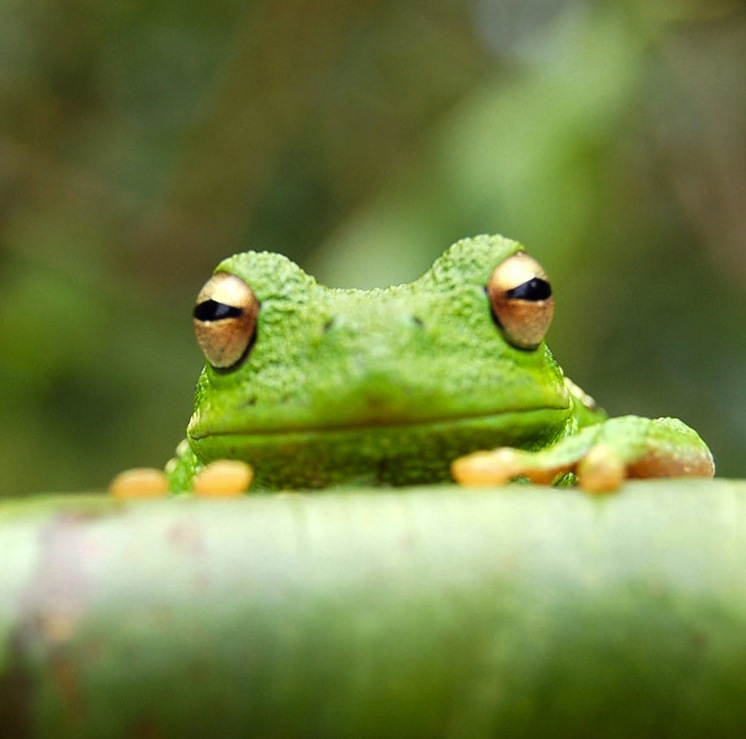
\includegraphics[width=\linewidth]{frog.jpg}
  \caption{\textbf{Description of the whole figure.} \textbf{(a)} Description of panel a. \textbf{(b)} ... Always include readable labels and units. Include uncertainty bands or error bars when appropriate. Check real Physical Review Letters papers for reference.}
  \label{fig:intro}
\end{figure}


% ---------- Section II ----------
\section{Background and Related Work}

\paragraph*{Physics background.} Summarize the essential theory (1--3 equations max) used later. For example, a damped oscillator:
\begin{equation}
m \ddot{x} + \gamma \dot{x} + k x = F(t).
\end{equation}

\paragraph*{Prior work.} Cite 5--10 papers, libraries or textbooks that informed your approach and data \cite{greenwade93,savvidis_resonant_2004,waschke_coherent_1993}.


% ---------- Section III ----------
\section{Data and Experimental/Simulation Setup}

\paragraph*{Data source(s).} Provide links and licenses where applicable. State formats (CSV, HDF5, FITS) and sizes.

\paragraph*{Preprocessing.} Filtering, normalization, detrending, feature engineering. Results are visualized in Fig.~\ref{fig:data}, for example.

\paragraph*{Train/validation/test.} Describe split strategy and rationale (e.g., stratified split, time-aware split).

\begin{figure}[h]
  \centering
  % Replace with your file; keep vector (PDF) if possible
  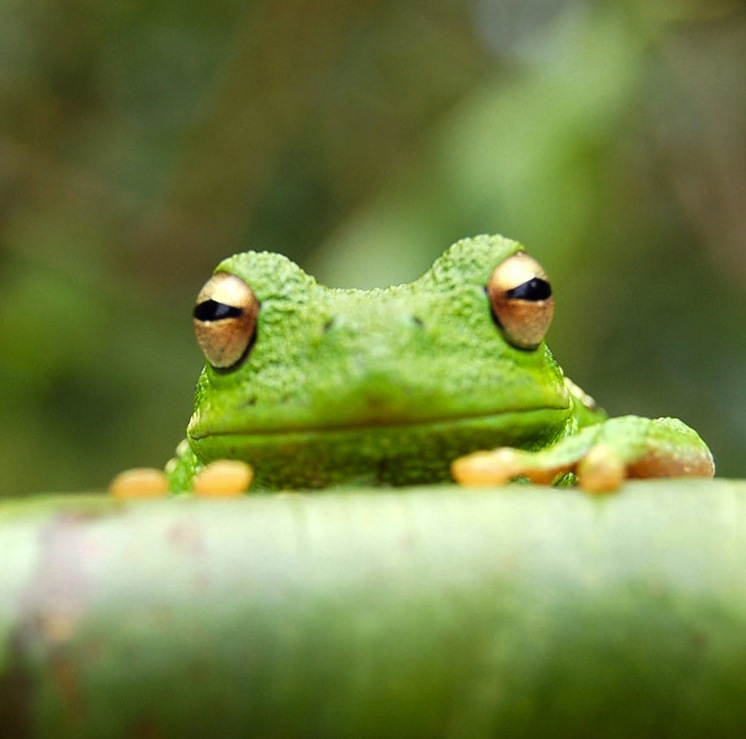
\includegraphics[width=\linewidth]{frog.jpg}
  \caption{Example captions.}
  \label{fig:data}
\end{figure}


% ---------- Section IV ----------
\section{Methods}

\paragraph*{Computational pipeline.} High-level steps from raw data to final result.

\paragraph*{Numerical/ML methods.} Be specific (e.g., Discrete Fourier Transform; windowing; zero-padding; SVM with RBF kernel; MLP with (40,40) tanh).

\paragraph*{Key equations.} Keep them readable; define symbols. For example, DFT magnitude (one-sided scaling for real signals):
\begin{equation}
\begin{aligned}
X_k &= \sum_{n=0}^{N-1} x_n e^{-i 2\pi kn / N}, \\
|X(f_k)|_{\text{one-sided}} &=
\begin{cases}
\frac{|X_k|}{N},  & k=0 \text{ or } k=N/2,\\
\frac{2|X_k|}{N}, & \text{otherwise}.
\end{cases}
\end{aligned}
\end{equation}

\paragraph*{Hyperparameters.} List values and how chosen (grid search, cross-validation).

\paragraph*{Code snippet.}
Some explanations

\begin{lstlisting}[language=Python, caption={Example: one-sided FFT magnitude in NumPy}]
import numpy as np
X = np.fft.rfft(x)              # rfft: real-to-complex, nonnegative freqs
f = np.fft.rfftfreq(len(x), d=dt)
mag = np.abs(X) / len(x)
if len(mag) > 2:
    mag[1:-1] *= 2              # double interior bins
\end{lstlisting}


% ---------- Section V ----------
\section{Results}

\subsection{Result I: Summary of first major result}
\paragraph*{Main findings.} State your primary quantitative results with units and uncertainties where possible.

\paragraph*{Figures.} Choose 2--4 plots that tell the story (label axes with units; readable legends). Cite the relevant figures in the texts (Fig.~\ref{fig:main_1})
\begin{figure}[h]
  \centering
  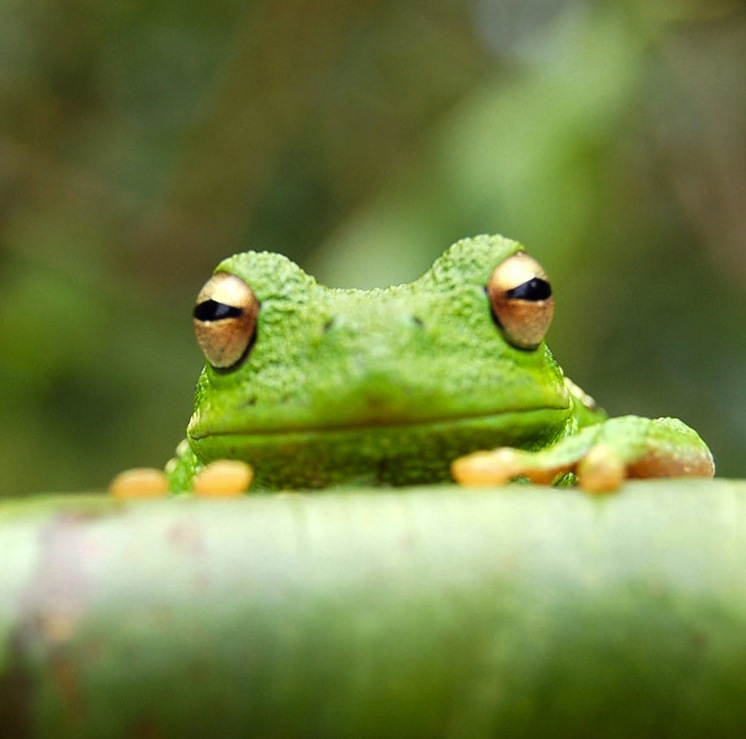
\includegraphics[width=\linewidth]{frog.jpg}
  \caption{\textbf{Result I: XXXX.} Main result plot with clear legend and units.}
  \label{fig:main_1}
\end{figure}

\subsection{Result II: Summary of 2nd major result}
Descriptions, plots, discussions, etc. Add more subsections if necessary. 

% ---------- Section VI ----------
\section{Discussions}

\paragraph*{Validations.} Compare against analytic baselines or known physical laws when available.

\paragraph*{Uncertainty.} Report confidence intervals, standard errors, or repeated-trial variation.

\paragraph*{Ablations.} What happens if you change a key setting (e.g., window type, train/test split)?

\paragraph*{Limitations.} Scope the conditions under which your approach may fail.


% ---------- Section VII ----------
\section{Computational Techniques, Reproducibility, and Code Availability}

\paragraph*{Environment.} OS, Python, and package versions (if applicable, put exact versions in \texttt{environment.yml}/\texttt{requirements.txt}).

\paragraph*{Repository.} Public GitHub with README instructions and a Jupyter notebook that directly runs when pulled into Datahub and recreates the results and figures for this report:
\begin{itemize}
  \item GitHub: \href{https://github.com/your-org/your-repo}{https://github.com/your-org/your-repo}
  \item How to run: notebook and/or commands to reproduce figures
  \item Data access: links or generation scripts, should be in repo
\end{itemize}


\section{Conclusions and Future Work}

\paragraph*{} Summarize the physics insight and computational takeaways. List 1–2 concrete next steps.

\section*{Author Contributions}

\paragraph*{} Detailed account of who did what. 

\section*{Use of AI Tools (Disclosure)}

\paragraph*{} Describe if/how AI tools (e.g., ChatGPT, Copilot) were used for debugging, code comments, or prose, and how outputs were verified. Attribute any generated text or code you adopted.

% ---------- Acknowledgments ----------
\begin{acknowledgments}
Acknowledge data providers, mentors, GSIs, if any.
\end{acknowledgments}

% ---------- References ----------
\bibliographystyle{apsrev4-2}
\begingroup
{
\bibliography{sample.bib}}
\endgroup

\end{document}
